\documentclass[../main.tex]{subfiles}

\graphicspath{{../images/}}

% sum commands

\begin{document}

\setcounter{section}{1}
\begin{center}
    \addcontentsline{toc}{section}{Homework 2}
    \section*{Homework 2}
    \subsection*{Due 2/6 12pm}
\end{center}
\hrule \vspace{10px}

\paragraph*{1.}
\begin{align*}
    P(r | \lambda) = \exp(-\lambda) \frac{\lambda^r}{r!}
\end{align*}
(a) Taking the log of the likelihood function:
\begin{align*}
    L(\lambda) = \ln P(r | \lambda) = -\lambda + r \ln \lambda - \ln r!
\end{align*}
finding the maximum by taking the derivative with respect to $\lambda$ and setting it to zero:
\begin{align*}
    \frac{dL}{d\lambda} = -1 + \frac{r}{\lambda} = 0 \implies \hat \lambda = r
\end{align*}
so the maximum likelihood estimate for $\lambda$ is $\hat{\lambda} = r$.

(b) Given the derivative with respect to the function $\ln \lambda$:
\begin{align*}
    \dv{(\ln{\lambda})} u^n = nu^n, \qquad \dv{(\ln{\lambda})} \ln \lambda = 1
\end{align*}
we can find the curvature of the log likelihood function:
\begin{align*}
    \dv{(\ln \lambda)} L(\lambda) &= -\lambda + r = 0 \implies \hat \lambda = r \\
    \dv[2]{(\ln \lambda)} L(\lambda) &= -\lambda = k
\end{align*}
For a normal distribution with width $\sigma$, the curvature is $k = -1/\sigma^2$. So the width is
approximately
\begin{align*}
    \sigma \propto \frac{1}{\sqrt{-k}} = \frac{1}{\sqrt{\lambda}}
\end{align*}
and the 95\% confidence interval at the MLE is approximately
\begin{align*}
    \hat \lambda \pm 2\sigma = r \pm \frac{2}{\sqrt{\hat \lambda}}
\end{align*}
(c) Given the new Poisson distribution
\begin{align*}
    P(r | \lambda) = \exp(-(\lambda + b)) \frac{(\lambda + b)^r}{r!}
\end{align*}
the log likelihood function is
\begin{align*}
    L(\lambda) = -(\lambda + b) + r \ln(\lambda + b) - \ln r!
\end{align*}
and the maximum likelihood estimate for $\lambda$ is
\begin{align*}
    \frac{dL}{d\lambda} = -1 + \frac{r}{\lambda + b} = 0 \implies \hat \lambda = r - b
\end{align*}
the value $\hat \lambda = 9 - 13 = -4$ is not physically meaningful, so the MLE will be the lowest
possible value for $\lambda$ which is $\hat \lambda = 0$. From this we can infer that the remote 
star is very dim. The Bayesian posterior distribution for $\lambda$ is
\begin{align*}
    P(\lambda | r) = \frac{P(r | \lambda)P(\lambda)}{P(r)}
\end{align*}
and sketched in the figure below
\begin{figure*}[ht]
    \centering
    \includegraphics[width=0.4\textwidth]{hw2_1.png}
    \caption{The posterior distribution for $\lambda$ given $r$}
\end{figure*}

\paragraph*{2.}
\begin{figure}[ht]
    \centering
    \includegraphics[width=0.4\textwidth]{hw2_2a.png}
    \caption{Segment of Gaussian distribution at $\qt{x_1 , y_1}$}
    \label{fig:hw2_2}
\end{figure}
(a) From the geometric picture as shown in Figure \ref{fig:hw2_2}, the segment of the Gaussian 
is a circle with radius $\rho = \sqrt{x_1^2 + y_1^2}$ and the circumference is $2\pi \rho$ which
directly relates to the extra factor of $\rho$ and canceling the $2\pi$ in the denominator. This 
is also related to the Jacobian when transforming from Cartesian to polar coordinates when computing 
the integral. Using the integral of a 1D Gaussian:
\begin{align*}
    \int_{-\infty}^\infty \exp(-ax^2) \dd{x} = \sqrt{\frac{\pi}{a}}
\end{align*}
Verifying that the integral is normalized:
\begin{align*}
    \frac{1}{2\pi\sigma^2} \iint_{-\infty}^\infty \exp(-\frac{x^2 + y^2}{2\sigma^2}) \dd{x} \dd{y}
    &= \frac{1}{\sigma^2} \int_0^\infty \exp(-\frac{\rho^2}{2\sigma^2}) \rho \dd{\rho} \\
    \frac{1}{2\pi\sigma^2} \int_{-\infty}^\infty \exp(-\frac{x^2}{2\sigma^2}) \dd{x} 
        \int_{-\infty}^\infty \exp(-\frac{y^2}{2\sigma^2}) \dd{y}
    &= \frac{1}{\sigma^2}
        \int_0^\infty \exp(-\frac{\rho^2}{2\sigma^2}) \rho \dd{\rho} \\
    \frac{1}{2\pi\sigma^2} \sqrt{2\pi\sigma^2} \sqrt{2\pi\sigma^2}
    &= \frac{1}{\sigma^2} \int_0^\infty \sigma^2 \exp(-u) \dd{u} \\
    \frac{2\pi\sigma^2}{2\pi\sigma^2} &= \qt[-e^{-u}]\eval_0^\infty = 1
\end{align*}
so both integrals are normalized.

(b)
\begin{align*}
    P(\rho) = \frac{\rho}{\sigma_w^k} \exp(-\frac{\rho^2}{2\sigma_w^2})
\end{align*}
\begin{figure}[h]
    \centering
    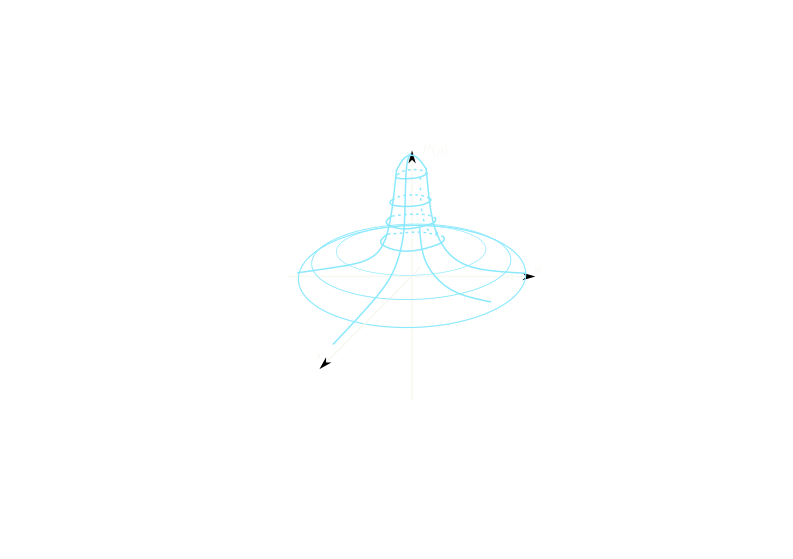
\includegraphics[width=0.5\textwidth]{hw2_2b.png}
    \caption{The distribution of $\rho$ for $k = 1000$}
    \label{fig:hw2_2b}
\end{figure}
The sketch for the distribution of $P(\rho)$ is shown in Figure \ref{fig:hw2_2b}.

(c) The standard deviation is
\begin{align*}
    \sigma_w = \sqrt{\frac{\sum (w - \mu)^2}{k}} 
\end{align*}
and because the distribution is centered at the origin, the mean is $\mu = 0$, so
\begin{align*}
    \sigma_w = \sqrt{\frac{\rho^2}{k}}
\end{align*}
Since most of the probability mass lies around $\rho$ or equivalently a radius of the thin shell
where $\rho = r = \sigma_w \sqrt{k}$, and the thickness of the shell is equivalent to the standard
deviation of the gaussian $ = r / \sqrt{k}$.

(d) Taking the ratio of the probability density from the origin to a point $\rho = \omega_w \sqrt k$
away:
\begin{align*}
    \frac{P(0)}{P(\sigma_w \sqrt k)} &= \exp{\frac{\sigma_w ^2 k}{2 \sigma_w^2 }} =\exp{\frac{k}{2}}
\end{align*}

(e) For a shell to contain 95\% of the probability mass, $\sigma_w = 2$ and thus the radius and 
thickness of the shell are
\begin{align*}
    r = \sigma_w \sqrt k = 2\sqrt{1000} = 63.25, \qquad \frac{r}{\sqrt{1000}} = 2
\end{align*}
and the probability density is $\exp{500} \approx 10^{217}$ larger at the origin than at the edge
of the shell.

(f) For a 1\% difference in $\sigma_w$ at the origin, the radius term is at zero so the exponents 
are 1, so the ratio of the probability densities is
\begin{align*}
    \frac{(1.01\sigma_w)^k}{\sigma_w^k} = 1.01^{k} \approx 20959.
\end{align*}

(g) Because of the large amount of parameters, the MLE would have an expected value at where the
probability density is the largest, which is at the origin, but as we have seen, the probability 
mass is almost all at the edge of the thin shell of radius $\sigma_w \sqrt k$. The narrow peak 
at the origin will overwhelm the MLE and thus we don't see the full picture of the distribution.

\newpage
\paragraph*{3.} 

(a) From class
\begin{align*}
    \mathcal{R} &= \frac{\frac{F_a! F_b!}{(F + 1)!}}{1/2^{F}} 
        = \frac{2^{F} F_a! F_b!}{(F + 1)!}
\end{align*}

(b) Taking the log of the ratio and using Stirling's approximation as shown in the code we get the
plot of the three simulations in Figure \ref{fig:hw2_3b}

\begin{figure*}[ht]
    \centering
    \includegraphics[width=0.5\textwidth]{hw2_3b.png}
    \caption{The log of the ratio of the likelihoods for the three simulations}
    \label{fig:hw2_3b}
\end{figure*}

(c) The trajectory of the two biased coin models are shown in Figure \ref{fig:hw2_3c1} and \ref{fig:hw2_3c2}.

\begin{figure}[h!]
    \centering
    \begin{minipage}{0.5\textwidth}
        \centering
        \includegraphics[width=0.8\linewidth]{hw2_3c1.png}
        \captionsetup{width=0.8\linewidth}
        \caption{There isn't clear evidence for a bias in the first 200 flips}
        \label{fig:hw2_3c1}
    \end{minipage}%
    \begin{minipage}{0.5\textwidth}
        \centering
        \includegraphics[width=0.8\linewidth]{hw2_3c2.png}
        \captionsetup{width=0.8\linewidth}
        \caption{A clear bias is shown in the first 200 flips here}
        \label{fig:hw2_3c2}
    \end{minipage}
\end{figure}

and the posterior distribution for the two biased coin models are shown in Figure \ref{fig:hw2_3d1}
and \ref{fig:hw2_3d2}.

\begin{figure*}[ht]
    \centering
    \begin{minipage}{0.5\textwidth}
        \centering
        \includegraphics[width=0.8\textwidth]{hw2_3d1.png}
        \captionsetup{width=0.8\linewidth}
        \caption{We can see that the distribution is centered around roughly $p_a = 0.55$ as expected}
        \label{fig:hw2_3d1}
    \end{minipage}%
    \begin{minipage}{0.5\textwidth}
        \centering
        \includegraphics[width=0.8\textwidth]{hw2_3d2.png}
        \captionsetup{width=0.8\linewidth}
        \caption{There is definitely a bias towards $p_a = 0.9$ in this distribution}
        \label{fig:hw2_3d2}
    \end{minipage}
\end{figure*}

\newpage
(d) From the Gaussian, we can approximate the error bars as $p_a - \frac{1}{2}$, so
\begin{align*}
    p_a - 0.5 = \frac{\sigma}{\sqrt{F}} \to F = \frac{\sigma^2}{(p_a - 0.5)^2}
\end{align*}
so we can get a rough estimate of the number of flips needed to distinguish between the two models
for within 2-3 standard deviations as shown in \ref{fig:hw2_3e1} and \ref{fig:hw2_3e2}.

\begin{figure}[ht]
    \centering
    \begin{minipage}{0.5\textwidth}
        \centering
        \includegraphics[width=0.8\textwidth]{hw2_3e1.png}
        \captionsetup{width=0.8\linewidth}
        \caption{For $\sigma = 3$ the model is clearly distinguishable after $\approx 3600$ flips}
        \label{fig:hw2_3e1}
    \end{minipage}%
    \begin{minipage}{0.5\textwidth}
        \centering
        \includegraphics[width=0.8\textwidth]{hw2_3e2.png}
        \captionsetup{width=0.8\linewidth}
        \caption{For $sigma = 2$ the model does seem to to be biased, but it is not as confident as the
        previous case}
        \label{fig:hw2_3e2}
    \end{minipage}
\end{figure}

(e) It is suprising to find out that finding evidence against $\mathcal{H}_1$ would be slower than
finding evidence for it, but in hindsight it makes sense for cases where the biased probabilities 
are close to the unbiased coin model since we would need an exponential number of flips as the bent
coin model probabilities is closer to $p_o = 1/2$. 

From the log of the ratio
\begin{align*}
    \ln \mathcal{R} &= F \ln 2 + \ln F_a! + \ln F_b! - \ln (F + 1)! \\
    &= F \ln 2 + \ln (F - F_b)! + \ln (F - F_a)! - \ln (F + 1)! \\
    &= F \ln 2 + (F - F_b) \ln (F - F_b) - (F - F_b) + \frac{1}{2} \ln 2\pi(F - F_b)\dots
\end{align*}
taking the derivative
\begin{align*}
    \dv{F} \ln \mathcal{R} &= \ln 2 + 1 + \ln (F - F_b) - 1 + \frac{1}{2} \frac{1}{F - F_b}\dots \\
    &= \ln 2 + \ln (F_a) + \frac{1}{2 F_a} + \ln (F_b) + \frac{1}{2 F_b}
        - \ln (F + 1) - \frac{1}{2 (F + 1)} 
\end{align*}

The fastest $\log \mathcal{R}$ can grow is when $F$ is very large, and the fractional terms at very
large $F$ will be negligible and the log terms grow much slower (e.g. $\ln(10^{20}) \approx 46$),
so the derivative will be be approximately a constant which relates to a linear growth.
The fastest $\log \mathcal{R}$ can fall is when $F$ is small and where the $-\ln(F + 1)$ term will
dominate thus the growth will be approximately logarithmic.


\newpage
\section*{PYTHON CODE BELOW}

\lstinputlisting[language=Python]{../code/hw2.py}

\end{document}
